\clearpage
\section{Event Selections}
\label{sec:selections}
The process under investigation is $e^{+} e^{-} \rightarrow \pip\pim\piz \gamma_{\mathrm{ISR}}$, whose final states include two charged tracks, one neutral $\piz$, and one ISR photon. The following selection criteria is applied to all the data samples. Here the figures are shown by taking $\sqrt{s}=3.773 \mathrm{GeV}$ round16 data as an example. The distributions related to the event selection of other data sets are shown in Appendix. XXX. Situations are similar to each other.


\begin{itemize}
    \item Good charged track:
          A charged track is taken as a good MDC track if it originates from the beam vertex and lies within the MDC polar angle region:
          \begin{itemize}
              \item $|\cos\theta|<0.93$, where $\theta$ is the polar angle with respect to the beam axis.
              \item $|\Delta r|<1\,\unit{cm}$, $|\Delta z|<10\,\unit{cm}$, where $|\Delta r|$ and $|\Delta z|$ is distance of closest approach to the interaction point (IP) perpendicular to the beam axis and along the beam axis, respectively.
              \item  the ratio of the calorimeter-deposited energy to the track momentum $E_{EMC}/p$ is required to be less than 0.8 for both of the charged tracks.
              \item no PID requirements for $\pip$, $\pim$.
          \end{itemize}

          % \item PID requirement:
          %       d$E$/d$x$ and TOF informations are combined to form the PID confidence level for protons, pions and kaons, respectively. $p^\pm$ is identified with:
          %       \begin{itemize}
          %           \item $p$ PID requirements: $\mathcal{L}$($p$)$>$0 $\mathcal{\&\&}$ $\mathcal{L}$($p$)$>$$\mathcal{L}$($K$) $\mathcal{\&\&}$ $\mathcal{L}$($p$)$>$$\mathcal{L}$($\pi$).
          %                 %   \item $K$ PID requirements: prob($K$)$>$0 $\mathcal{\&\&}$ prob($K$)$>$prob($\pi$).
          %                 %   \item $\pi$ PID requirements:  prob($\pi$)$>$0 $\mathcal{\&\&}$ prob($\pi$)$>$prob($K$).
          %       \end{itemize}

    \item $\gamma$ selection:
          \begin{itemize}
              \item $E>0.025\gev$~(barrel: $|\cos\theta|<0.8$), $E>0.050\gev$~(endcap: $0.86<|\cos\theta|<0.92$).
              \item $0\leqslant t_{\rm TDC} \leqslant 14$($\times 50 \unit{ns}$) to suppress fake photons due to electronic noise or beam background.
              \item the closest angle with all charged tracks $\theta>10^{\circ}$ to suppress background from radiation of charged tracks.
          \end{itemize}
    \item $\piz \to \gamma\gamma$ selection:
          \begin{itemize}
              \item two photon invariant mass $M_{\gamma\gamma}$ within (0.115, 0.150)$\gevcc$.
              \item To improve the momentum resolution, 1C kinematic fit is performed. Here, the 1C means $\piz$ mass constraint, and the updated 4-momentum will be used in the further analysis. $\chi^2_{\mathrm{KF}}<10$
          \end{itemize}
\end{itemize}

Candidate events are selected by requiring exactly two good charged tracks, accompanied by at least one reconstructed $\pi^0$ and a minimum of three good photon showers. This ensures the presence of at least one $\pi^0$ and one isolated photon from Initial-State Radiation ($\gamma_{\mathrm{ISR}}$). A four-constraint (4C) kinematic fit is then applied to the event, and the candidate with the smallest $\chi_{\mathrm{4C}}^2$ value is chosen for further analysis.

After identifying an ISR photon from the isolated photon showers, the invariant mass of the remaining $e^+e^- \to \pi^+\pi^-\pi^0$ system is reconstructed. As expected for ISR processes, the resulting center-of-mass energy $\sqrt{s'}$ of the $\pi^+\pi^-\pi^0$ system shows a continuous spectrum, characteristic of the radiative return mechanism. This continuum behavior is illustrated in Fig.~\ref{fig:signal_mc_mass_spectra} across the $\omega(782)$, $\phi(1020)$, and $\omega^{\prime}/\omega^{\prime\prime}$ mass regions.

\begin{figure}[H]
    \centering
    \subfloat[$\omega(782)$ region]{
        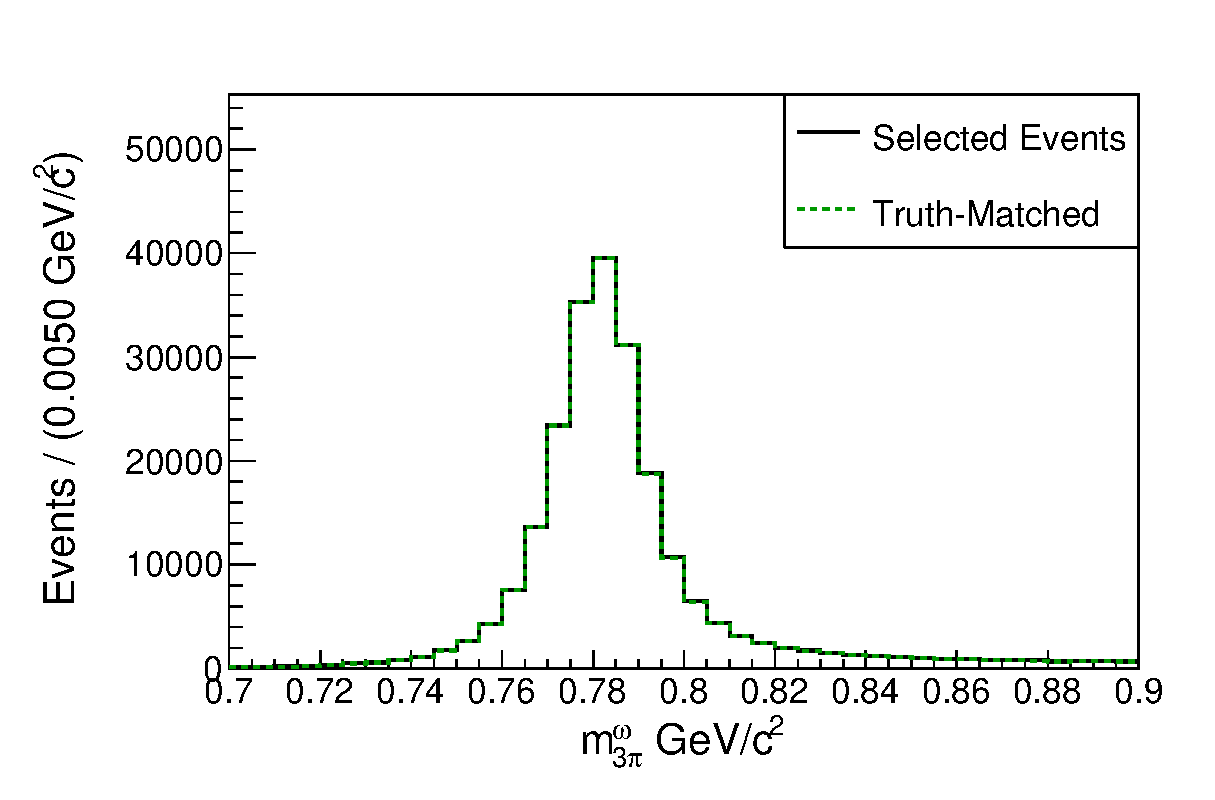
\includegraphics[width=0.32\textwidth]{fig/hist_omega_region_with_truth.eps}
        \label{fig:mc_mass_omega_region}
    }
    \hfill
    \subfloat[$\phi(1020)$ region]{
        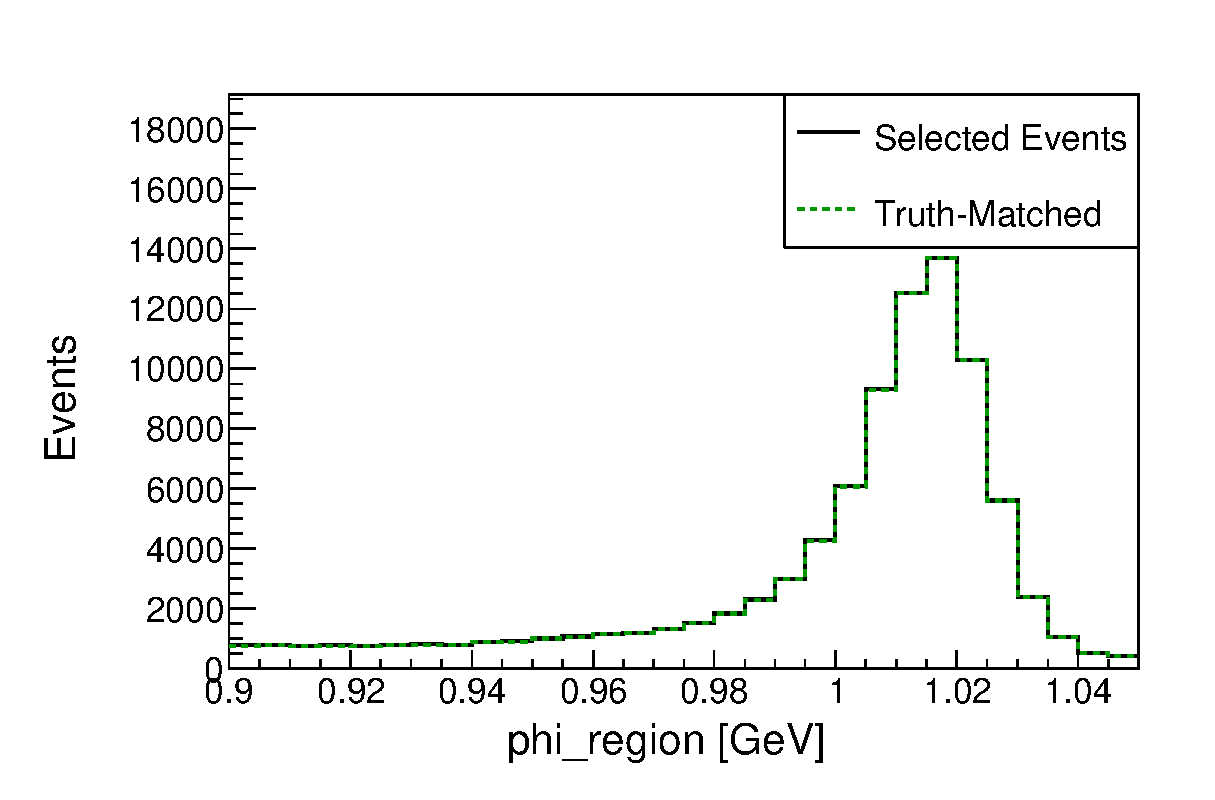
\includegraphics[width=0.32\textwidth]{fig/hist_phi_region_with_truth.eps}
        \label{fig:mc_mass_phi_region}
    }
    \hfill
    \subfloat[$\omega^{\prime}$ and $\omega^{\prime\prime}$ region]{
        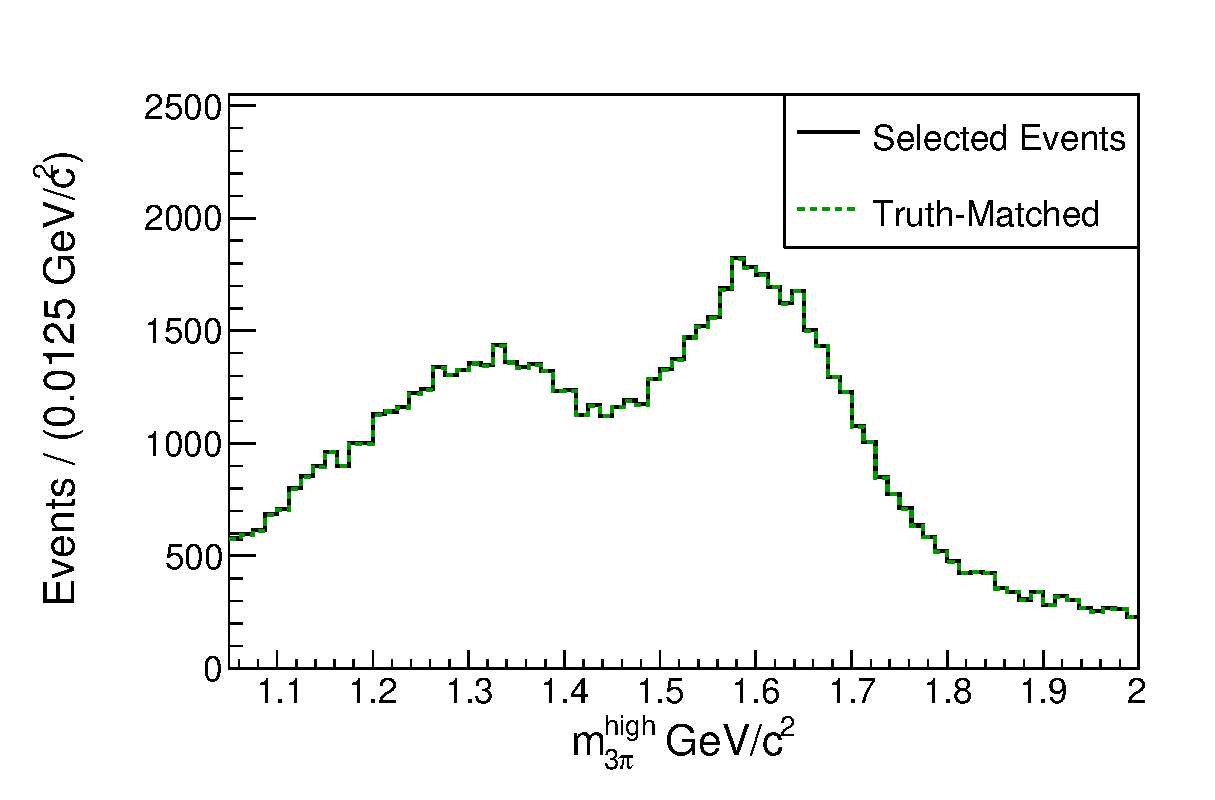
\includegraphics[width=0.32\textwidth]{fig/hist_omegap_region_with_truth.eps}
        \label{fig:mc_mass_omegap_region}
    }

    \caption{Invariant mass spectra of MC in the (a) $\omega(782)$, (b) $\phi(1020)$, and (c) $\omega^{\prime}/\omega^{\prime\prime}$ mass regions. The distributions correspond to $M(pK_S^0)$, $M(p\pi^0)$, and $M(K_S^0\pi^0)$, respectively. The "Truth-Matched" distribution (green dashed line) corresponds to reconstructed events where the momentum directions of the $\pi^0$ and $\gamma_{\mathrm{ISR}}$ successfully match their truth-level counterparts. A loose requirement of $\chi^2_{\text{KF}} < 100$ is applied to the kinematic fit. The continuous spectrum of $\sqrt{s'}$ for the $\pi^+\pi^-\pi^0$ system demonstrates the radiative return mechanism via ISR. }
    \label{fig:signal_mc_mass_spectra}
\end{figure}